%
% grad4.tex
%
% (c) 2018 Prof Dr Andreas Müller, Hochschule Rapperswil
%
\documentclass[tikz]{standalone}
\usepackage{times}
\usepackage{amsmath}
\usepackage{txfonts}
\usepackage[utf8]{inputenc}
\usepackage{graphics}
\usetikzlibrary{arrows,intersections,math}
\begin{document}

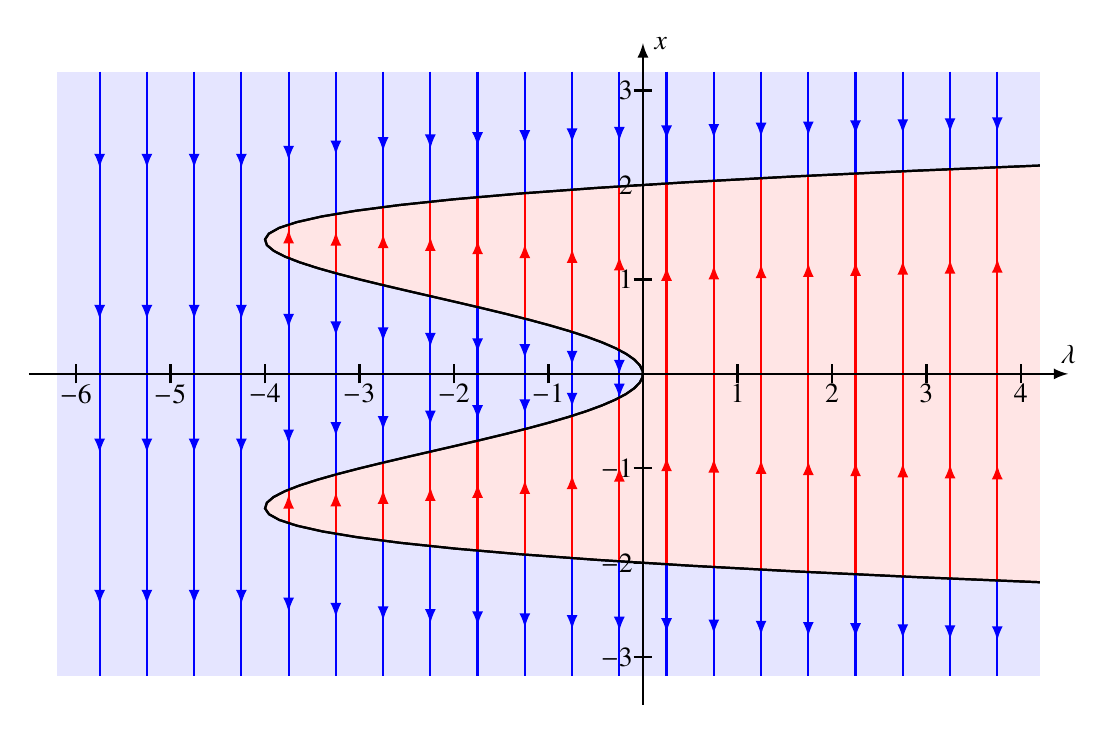
\begin{tikzpicture}[>=latex,thick,scale=1.2]

\def\wl{-6.2}
\def\wr{4.2}
\def\h{3.2}
\def\s{0.13}

\pgfmathparse{sqrt(2+sqrt(6))}
\edef\l{\pgfmathresult}

\begin{scope}
\clip ({\wl},{-\h}) rectangle ({\wr},{\h});
\fill[color=blue!10] ({\wl},{-\h})--({\wr},{-\h})--({\wr},{\h})--({\wl},{\h})
	--cycle;

\fill[color=red!10,domain=-3:3,samples=100]
	plot ({\x*\x*(\x*\x-4)},{\x})--cycle;
\draw[domain=-3:3,samples=100] plot ({\x*\x*(\x*\x-4)},{\x});

\end{scope}

\tikzmath{
	real \xtop, \xabove, \xbelow, \xbottom;
	\xtop = (\h + sqrt(2))/2;
	\xabove = sqrt(2)/2;
	\xbelow = -\xabove;
	\xbottom = -\xtop;
}

\foreach \l in {-5.75,-5.25,...,-4.25}{
	\draw[->,color=blue] ({\l},{\h})--({\l},{\xtop-\s});
	\draw[->,color=blue] ({\l},{\xtop})--({\l},{\xabove-\s});
	\draw[->,color=blue] ({\l},{\xabove})--({\l},{\xbelow-\s});
	\draw[->,color=blue] ({\l},{\xbelow})--({\l},{\xbottom-\s});
	\draw[color=blue] ({\l},{\xbottom})--({\l},{-\h});
}

\foreach \l in {-3.75,-3.25,...,-0.25}{
	\tikzmath{
		real \xplus, \xminus, \xtop, \xabove, \xbelow, \xbottom;
		\xplus = sqrt(2 + sqrt(4 + \l));
		\xminus = sqrt(2 - sqrt(4 + \l));
		\xtop = (\h + \xplus)/2;
		\xabove = \xminus/2;
		\xbelow = -\xabove;
		\xbottom = -\xtop;
	}
	\draw[->,color=blue] ({\l},{\h})--({\l},{\xtop-\s});
	\draw[color=blue] ({\l},{\xtop})--({\l},{\xplus});

	\draw[->,color=blue] ({\l},{\xminus})--({\l},{\xabove-\s});
	\draw[->,color=blue] ({\l},{\xabove})--({\l},{\xbelow-\s});
	\draw[color=blue] ({\l},{\xbelow})--({\l},{-\xminus});

	\draw[->,color=blue] ({\l},{-\xplus})--({\l},{\xbottom-\s});
	\draw[color=blue] ({\l},{\xbottom})--({\l},{-\h});

	\draw[->,color=red] ({\l},{\xminus})--({\l},{(\xplus+\xminus)/2+\s});
	\draw[color=red] ({\l},{(\xplus+\xminus)/2})--({\l},{\xplus});

	\draw[->,color=red] ({\l},{-\xplus})--({\l},{-(\xplus+\xminus)/2+\s});
	\draw[color=red] ({\l},{-(\xplus+\xminus)/2})--({\l},{-\xminus});
}

\foreach \l in {0.25,0.75,...,3.75}{
	\tikzmath{
		real \xupper, \xlower;
		\xupper = sqrt(2 + sqrt(4 + \l));
		\xlower = -\xupper;
	}
	\draw[->,color=red] ({\l},{\xlower})--({\l},{\xlower/2 +\s});
	\draw[->,color=red] ({\l},{\xlower/2})--({\l},{\xupper/2+\s});
	\draw[color=red] ({\l},{\xupper/2})--({\l},{\xupper});
	\draw[->,color=blue] ({\l},{\xlower})--({\l},{(\xlower-\h)/2-\s});
	\draw[color=blue] ({\l},{(\xlower-\h)/2})--({\l},{-\h});
	\draw[->,color=blue] ({\l},{\h})--({\l},{(\xupper+\h)/2-\s});
	\draw[color=blue] ({\l},{(\xupper+\h)/2})--({\l},{\xupper});
}

\draw[->] ({\wl-0.3},0)--({\wr+0.3},0) coordinate[label=$\lambda$];
\draw[->] (0,{-\h-0.3})--(0,{\h+0.3}) coordinate[label={right:$x$}];

\begin{scope}
\clip ({\wl},{-\h}) rectangle ({\wr},{\h});
\draw[domain=-3:3,samples=100] plot ({\x*\x*(\x*\x-4)},{\x});
\end{scope}

\foreach \l in {-6,-5,-4,-3,-2,-1,1,2,3,4}{
	\draw ({\l},-0.1)--({\l},0.1);
	\node at ({\l},-0.0) [below] {$\l$};
}

\foreach \x in {-3,-2,-1,1,2,3}{
	\draw (-0.1,{\x})--(0.1,{\x});
	\node at (-0.0,{\x}) [left] {$\x$};
}

\end{tikzpicture}

\end{document}
